\documentclass[tikz,border=4pt]{standalone}
\usepackage{amsmath,amssymb}
\usetikzlibrary{positioning,arrows.meta,fit,backgrounds,calc}
\definecolor{cA}{HTML}{2A78D6}  % model / problem
\definecolor{cB}{HTML}{6E6E6E}  % critique
\definecolor{cC}{HTML}{D6477F}  % design
\definecolor{cD}{HTML}{E06A2B}  % security
\definecolor{cE}{HTML}{159A6B}  % evaluation
\definecolor{cF}{HTML}{7B4FB8}  % network science
\tikzset{
  stage/.style={draw=#1, line width=0.9pt, rounded corners=3pt, fill=#1!6, inner xsep=5pt, inner ysep=6pt},
  box/.style={draw=#1!85!black, rounded corners=2pt, fill=white, align=center, font=\scriptsize,
              inner sep=3pt, minimum height=7mm},
  title/.style={font=\bfseries\small, text=#1!80!black, anchor=south west, inner sep=2pt},
  arr/.style={-{Stealth[length=2.3mm]}, line width=0.9pt, draw=black!70},
  lab/.style={font=\scriptsize\itshape, text=black!70, align=center},
}
\hyphenpenalty=10000
\exhyphenpenalty=10000
\begin{document}
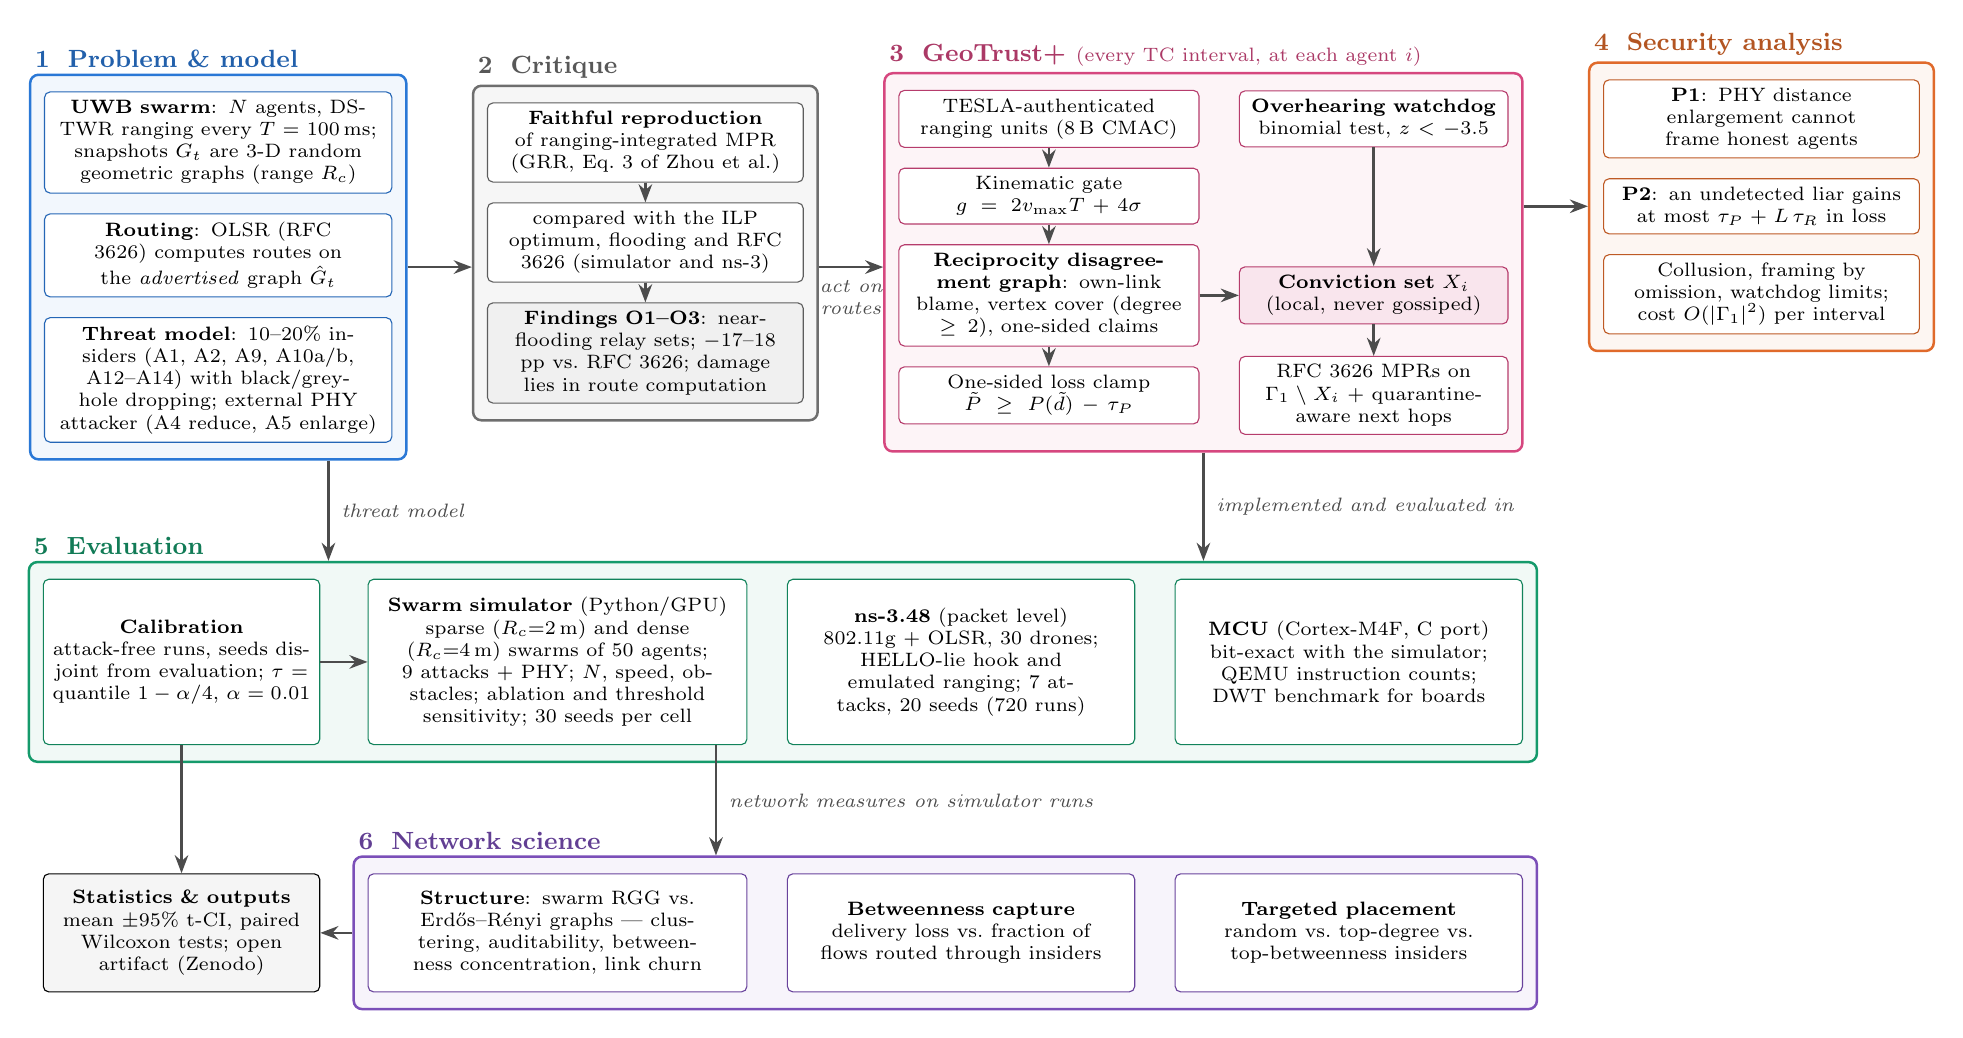
\begin{tikzpicture}[node distance=2.5mm]

%% ================================================================ row 1
%% 1. problem and model
\node[box=cA, text width=42mm] (m1) {\textbf{UWB swarm}: $N$ agents, DS-TWR ranging every $T=100$\,ms; snapshots $G_t$ are 3-D random geometric graphs (range $R_c$)};
\node[box=cA, text width=42mm, below=of m1] (m2) {\textbf{Routing}: OLSR (RFC 3626) computes routes on the \emph{advertised} graph $\hat G_t$};
\node[box=cA, text width=42mm, below=of m2] (m3) {\textbf{Threat model}: 10--20\% insiders (A1, A2, A9, A10a/b, A12--A14) with black/grey-hole dropping; external PHY attacker (A4 reduce, A5 enlarge)};
\begin{scope}[on background layer]
\node[stage=cA, fit=(m1)(m3)] (S1) {};
\end{scope}
\node[title=cA] at (S1.north west) {1\; Problem \& model};

%% 2. critique
\node[box=cB, text width=38mm, right=12mm of m1] (c1) {\textbf{Faithful reproduction}\\ of ranging-integrated MPR\\ (GRR, Eq.~3 of Zhou et al.)};
\node[box=cB, text width=38mm, below=of c1] (c2) {compared with the ILP optimum, flooding and RFC 3626 (simulator and ns-3)};
\node[box=cB, text width=38mm, below=of c2, fill=cB!10] (c3) {\textbf{Findings O1--O3}: near-flooding relay sets; $-$17--18 pp vs.\ RFC 3626; damage lies in route computation};
\draw[arr] (c1) -- (c2); \draw[arr] (c2) -- (c3);
\begin{scope}[on background layer]
\node[stage=cB, fit=(c1)(c3)] (S2) {};
\end{scope}
\node[title=cB] at (S2.north west) {2\; Critique};

%% 3. GeoTrust+ per-interval pipeline
\node[box=cC, text width=36mm, right=12mm of c1, yshift=3mm] (d1) {TESLA-authenticated\\ ranging units (8\,B CMAC)};
\node[box=cC, text width=36mm, below=of d1] (d2) {Kinematic gate\\ $g=2v_{\max}T+4\sigma$};
\node[box=cC, text width=36mm, below=of d2] (d3) {\textbf{Reciprocity disagreement graph}: own-link blame, vertex cover (degree $\ge2$), one-sided claims};
\node[box=cC, text width=36mm, below=of d3] (d4) {One-sided loss clamp\\ $\tilde P\ge P(\tilde d)-\tau_P$};
\node[box=cC, text width=32mm, right=5mm of d1] (d5) {\textbf{Overhearing watchdog}\\ binomial test, $z<-3.5$};
\node[box=cC, text width=32mm, fill=cC!14] at (d5 |- d3) (d6) {\textbf{Conviction set} $X_i$\\ (local, never gossiped)};
\node[box=cC, text width=32mm] at (d5 |- d4) (d7) {RFC 3626 MPRs on $\Gamma_1\setminus X_i$ + quarantine-aware next hops};
\draw[arr] (d1) -- (d2); \draw[arr] (d2) -- (d3); \draw[arr] (d3) -- (d4);
\draw[arr] (d3) -- (d6);
\draw[arr] (d5) -- (d6); \draw[arr] (d6) -- (d7);
\begin{scope}[on background layer]
\node[stage=cC, fit=(d1)(d4)(d5)(d7)] (S3) {};
\end{scope}
\node[title=cC] at (S3.north west) {3\; GeoTrust+ \normalfont\scriptsize(every TC interval, at each agent $i$)};

%% 4. security analysis
\node[box=cD, text width=38mm, right=12mm of d5] (s1) {\textbf{P1}: PHY distance enlargement cannot frame honest agents};
\node[box=cD, text width=38mm, below=of s1] (s2) {\textbf{P2}: an undetected liar gains at most $\tau_P+L\,\tau_R$ in loss};
\node[box=cD, text width=38mm, below=of s2] (s3) {Collusion, framing by omission, watchdog limits; cost $O(|\Gamma_1|^2)$ per interval};
\begin{scope}[on background layer]
\node[stage=cD, fit=(s1)(s3)] (S4) {};
\end{scope}
\node[title=cD] at (S4.north west) {4\; Security analysis};

%% row-1 flow
\coordinate (yflow) at ($(S1.north)!0.5!(S1.south)$);
\draw[arr] (S1.east |- yflow) -- (S2.west |- yflow);
\draw[arr] (S2.east |- yflow) -- node[lab, below=1pt]{act on\\ routes} (S3.west |- yflow);
\draw[arr] (S3.east |- s2) -- (S4.west |- s2);

%% ================================================================ row 2: evaluation
\coordinate (row2) at ($(S1.west |- S3.south)+(5pt,-16mm)$);
\node[box=cE, text width=33mm, minimum height=21mm, anchor=north west] (e0) at (row2)
  {\textbf{Calibration}\\ attack-free runs, seeds disjoint from evaluation; $\tau$ = quantile $1-\alpha/4$, $\alpha=0.01$};
\node[box=cE, text width=46mm, minimum height=21mm, anchor=north west] (e1) at ($(e0.north east)+(6mm,0)$)
  {\textbf{Swarm simulator} (Python/GPU)\\ sparse ($R_c{=}2$\,m) and dense ($R_c{=}4$\,m) swarms of 50 agents; 9 attacks + PHY; $N$, speed, obstacles; ablation and threshold sensitivity; 30 seeds per cell};
\node[box=cE, text width=42mm, minimum height=21mm, anchor=north west] (e2) at ($(e1.north east)+(5mm,0)$)
  {\textbf{ns-3.48} (packet level)\\ 802.11g + OLSR, 30 drones; HELLO-lie hook and emulated ranging; 7 attacks, 20 seeds (720 runs)};
\node[box=cE, text width=42mm, minimum height=21mm, anchor=north west] (e3) at ($(e2.north east)+(5mm,0)$)
  {\textbf{MCU} (Cortex-M4F, C port)\\ bit-exact with the simulator; QEMU instruction counts; DWT benchmark for boards};
\draw[arr] (e0) -- (e1);
\begin{scope}[on background layer]
\node[stage=cE, fit=(e0)(e3)] (S5) {};
\end{scope}
\node[title=cE] at (S5.north west) {5\; Evaluation};

%% ================================================================ row 3: network science + outputs
\coordinate (row3) at ($(e1.west |- S5.south)+(0,-14mm)$);
\node[box=cF, text width=46mm, minimum height=15mm, anchor=north west] (n1) at (row3)
  {\textbf{Structure}: swarm RGG vs.\ Erd\H{o}s--R\'enyi graphs --- clustering, auditability, betweenness concentration, link churn};
\node[box=cF, text width=42mm, minimum height=15mm, anchor=north west] (n2) at ($(n1.north east)+(5mm,0)$)
  {\textbf{Betweenness capture}\\ delivery loss vs.\ fraction of flows routed through insiders};
\node[box=cF, text width=42mm, minimum height=15mm, anchor=north west] (n3) at ($(n2.north east)+(5mm,0)$)
  {\textbf{Targeted placement}\\ random vs.\ top-degree vs.\ top-betweenness insiders};
\begin{scope}[on background layer]
\node[stage=cF, fit=(n1)(n3)] (S6) {};
\end{scope}
\node[title=cF] at (S6.north west) {6\; Network science};

\node[box=black, text width=33mm, minimum height=15mm, fill=black!4, anchor=north west] (o1) at (e0.west |- n1.north)
  {\textbf{Statistics \& outputs}\\ mean $\pm$95\% t-CI, paired Wilcoxon tests; open artifact (Zenodo)};

%% cross-row flows
\coordinate (tA) at ($(S1.south)+(14mm,0)$);
\draw[arr] (tA) -- node[lab, right=1pt]{threat model} (tA |- S5.north);
\draw[arr] (S3.south) -- node[lab, right=1pt]{implemented and evaluated in} (S3.south |- S5.north);
\coordinate (tB) at ($(e1.south east)+(-4mm,0)$);
\draw[arr] (tB) -- node[lab, right=1pt]{network measures on simulator runs} (tB |- S6.north);
\draw[arr] (S6.west |- n1) -- (o1.east);
\draw[arr] (e0.south) -- (o1.north);

\end{tikzpicture}
\end{document}
